% =====================================================================
\chapter{Por que analisar algoritmos?}\label{cap:01}
\naaula{04 e 05}

Desde a Aula 1, usamos expressões como \enquote{acesso por índice é $O(1)$} e \enquote{inserir no
início da lista contígua é $O(n)$}. Neste capítulo você vai entender \emph{por que} precisamos
desse tipo de medida e por que ela não é dada em segundos.

\begin{conexao}
Esta é a tabela que abriu o nosso curso, na Aula 1. Ao final desta apostila, você vai saber
explicar cada célula dela — e calcular tabelas como essa sozinho.

\begin{center}
\begin{tabularx}{0.86\linewidth}{L C C}
\cab \tc{Operação} & \tc{Contígua (array)} & \tc{Encadeada (lista)} \\
Acesso por índice & $O(1)$ & $O(n)$ \\
\rowcolor{white} Inserir/remover no início & $O(n)$ & $O(1)$ \\
Inserir/remover no fim & $O(1)$ & $O(1)$ \\
\end{tabularx}
\end{center}
\end{conexao}

\section{O mesmo problema, duas soluções}

Considere um problema simples: somar todos os números de 1 até $n$. Eis duas soluções corretas,
que sempre dão a mesma resposta:

\begin{lstlisting}
def soma_com_laco(n):
    total = 0
    for i in range(1, n + 1):   # repete n vezes
        total = total + i
    return total

def soma_com_formula(n):
    return n * (n + 1) // 2     # sempre 3 contas: *, + e //
\end{lstlisting}

Para $n = 10$, as duas devolvem 55 num piscar de olhos. Mas repare no trabalho de cada uma:
\codigo{soma_com_laco} faz uma soma para cada número — para $n$ igual a um bilhão, um bilhão de
somas. Já \codigo{soma_com_formula} faz sempre as mesmas 3 contas, seja $n$ igual a 10 ou a um
bilhão. (A fórmula vem de um truque famoso, a \emph{soma de Gauss}, que você verá na seção~3.7.)

\begin{intuicao}
Dois algoritmos podem resolver o mesmo problema com esforços completamente diferentes. Analisar
um algoritmo é responder: \textbf{como o trabalho cresce quando a entrada cresce?} No primeiro,
o trabalho cresce junto com $n$; no segundo, fica sempre igual.
\end{intuicao}

\section{Por que o cronômetro engana}

A primeira ideia para comparar algoritmos é medir o tempo. Foi o que fizemos no exercício 14 da
Aula 1. O problema é que o tempo depende de muitas coisas além do algoritmo: o processador, a
linguagem, outros programas abertos, até a temperatura da máquina. O mesmo código leva tempos
diferentes em computadores diferentes — e até em duas execuções no mesmo computador.

Veja uma medição real, feita no computador onde esta apostila foi gerada: o mesmo algoritmo de
ordenação (o Insertion Sort, que estudaremos no capítulo 9), com o vetor em ordem inversa,
escrito em C e em Python.

\begin{figure}[!htb]
  \centering
  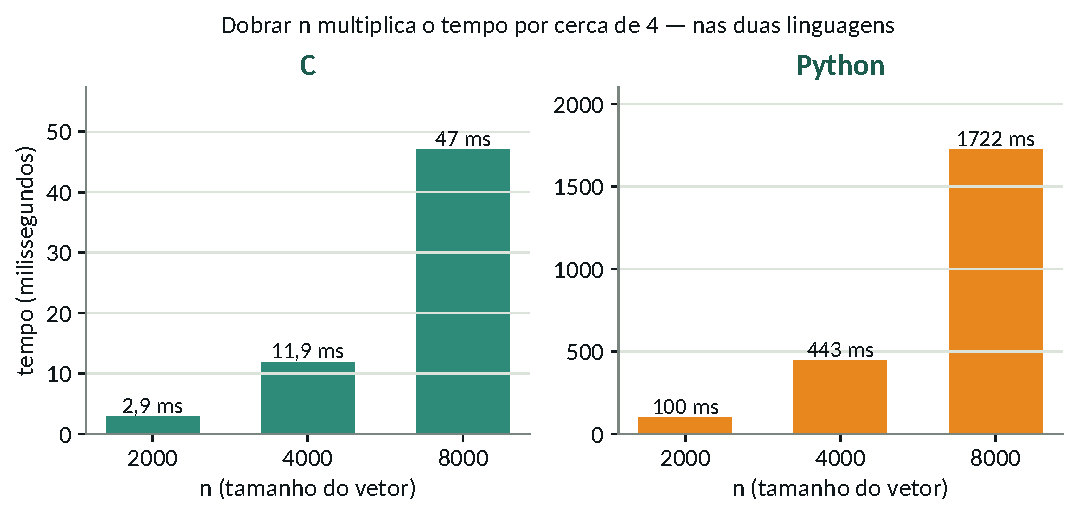
\includegraphics[width=0.92\textwidth]{figuras/f01_tempos_c_python.pdf}
  \caption{Tempo do mesmo algoritmo em C e em Python, para vetores de 2.000, 4.000 e 8.000
  elementos. Repare nas escalas: o Python é cerca de 35 vezes mais lento.}
\end{figure}

\begin{center}
\begin{tabularx}{0.8\textwidth}{L C C C}
\cab \tcx{$n$} & \tc{2.000} & \tc{4.000} & \tc{8.000} \\
Tempo em C & 2,9 ms & 11,9 ms & 47,0 ms \\
\rowcolor{edfundo} Tempo em Python & 100 ms & 443 ms & 1.722 ms \\
\textbf{Quanto multiplicou ao dobrar n} & — & $\approx 4\times$ & $\approx 4\times$ \\
\end{tabularx}
\end{center}

Os números absolutos são muito diferentes: 47 milissegundos contra quase 2 segundos. Mas o
\textbf{comportamento} é o mesmo nas duas linguagens: cada vez que $n$ dobra, o tempo fica cerca
de 4 vezes maior. Essa é a informação que vale em qualquer máquina e em qualquer linguagem — e é
ela que a análise de algoritmos captura.

\begin{atencao}
Os tempos da tabela vão mudar no seu computador. O \enquote{multiplicou por 4} não vai. É por
isso que, em vez de segundos, vamos medir algoritmos pelo \textbf{número de passos} e, mais
ainda, pela \textbf{forma como esse número cresce}.
\end{atencao}

\section{A ideia central: contar passos}

Em vez de cronometrar, vamos \textbf{contar} quantas operações simples o algoritmo executa em
função do tamanho da entrada, que chamaremos de $n$. O resultado é uma função, que escrevemos
como $T(n)$ — lê-se \enquote{tê de ene}. Por exemplo:

\begin{itemize}
  \item \codigo{soma_com_laco} faz um número de passos proporcional a $n$;
  \item \codigo{soma_com_formula} faz sempre o mesmo número de passos, não importa $n$.
\end{itemize}

Contar passos não depende da máquina: um computador mais rápido executa cada passo mais
depressa, mas a quantidade de passos é a mesma. No capítulo 2 você vai aprender a fazer essa
contagem com precisão, e nos capítulos seguintes, a resumir o resultado com as notações $O$,
$\Omega$ e $\Theta$.

\section{O caminho desta apostila}

\begin{center}
\begin{tabularx}{\textwidth}{P{3.2cm} L}
\cab \tc{Capítulos} & \tc{O que você vai aprender} \\
2 & contar os passos de um algoritmo e escrever $T(n)$ \\
\rowcolor{edfundo} 3 e 4 & a matemática necessária, do zero: funções, potências, logaritmos, somatórios, termo dominante \\
5, 6 e 7 & as notações $O$ (teto), $\Omega$ (piso) e $\Theta$ (justo) \\
\rowcolor{edfundo} 8 e 9 & melhor, pior e caso médio — com o Insertion Sort como estudo de caso \\
10 e 11 & comparar famílias de funções e usar derivadas para entender o crescimento \\
\rowcolor{edfundo} 12 e 13 & regras práticas para analisar código e a revisão das Aulas 1 a 3 \\
14 & o Campo Minado: regras, técnicas e análise de custo \\
\rowcolor{edfundo} 15 e 16 & lista de exercícios resolvidos e resumo para a prova \\
\end{tabularx}
\end{center}

\begin{exrapido}
Para $n = 1.000.000$, quantas somas \codigo{soma_com_laco} faz? E quantas contas faz
\codigo{soma_com_formula}? Se cada conta levasse 1 microssegundo, quanto tempo cada uma
levaria?
\end{exrapido}

\begin{respostas}
  \resp{1.1} \codigo{soma_com_laco} faz 1.000.000 de somas (uma por número), ou seja, cerca de
  1 segundo a 1 microssegundo por soma. \codigo{soma_com_formula} faz sempre 3 contas: cerca de
  3 microssegundos. E se $n$ fosse um bilhão, a primeira levaria uns 17 minutos; a segunda,
  os mesmos 3 microssegundos.
\end{respostas}
